% Fabrizio Margotta 789072
% Alma Mater Studiorum - Università di Bologna

\documentclass[a4paper]{article}

% \usepackage[toc,page]{appendix}
\usepackage[bookmarks]{hyperref}
\usepackage{graphicx}
\usepackage{float}
\usepackage{minted}
\usepackage{tikz}
\usepackage[nottoc]{tocbibind}
\usepackage{bookmark}
\graphicspath{{./img/}}
\hypersetup{pdftitle={Relazione di progetto-High Performance Computing},
    pdfauthor={Fabrizio Margotta},
    pdfkeywords={hpc, openmp, cuda}
}

\begin{document}

\title{Relazione di progetto\\
     Corso di High Performance Computing}
\author{Fabrizio Margotta
(\href{mailto:fabrizio.margotta@studio.unibo.it}{fabrizio.margotta@studio.unibo.it})\\
    Matricola 789072\\
    \\
  Alma Mater Studiorum-Università di Bologna\\}
% \subtitle{Programmazione di Reti - Progetto di gruppo}
\date{2019--08--24}

\maketitle \thispagestyle{empty}
\begin{abstract}
    TODO
\end{abstract}

\newpage \thispagestyle{empty}
%\begin{center}
%[Questa pagina è stata lasciata intenzionalmente bianca.]
%\end{center}
%\newpage
\setcounter{tocdepth}{2} % Show sections
\tableofcontents \thispagestyle{empty}

\newpage
\pagestyle{headings}

\section{Analisi}
L'analisi sul modello da implementare è stata particolarmente semplificata dalle
indicazioni fornite dal docente.

Vengono tuttavia di seguito presentate alcune osservazioni sul modello dei dati,
ad esempio si fa notare che non è presente alcuna particolare dipendenza sui
dati da parte delle iterazioni dei cicli.

Ciò permette quindi di procedere con la parallelizzazione della versione seriale
fornita senza particolari intoppi.

%\newpage
%\section{Design}

%\newpage
\section{Sviluppo}

\subsection{Ghost area}

Entrambe le soluzioni proposte si avvalgono dell'utilizzo di una ghost area
inizializzata a zero (e mai più modificata).

Ciò permette di ridurre notevolmente l'impatto sulle prestazioni
dell'operazione di propagazione, poiché, avendo una nuova regione di celle
intorno al dominio, non sarà più necessario controllare che le celle adiacenti a
quella presa in esame siano ai bordi del dominio stesso.
Il valore delle ghost cell (zero), inoltre, non influirà sui risultati delle
operazioni dell'algoritmo.

In figura \ref{fig:ghostarea}(\cite{marzollaghost}) è possibile osservare il
comportamento appena descritto.

\begin{figure}[!ht]
  \centering
  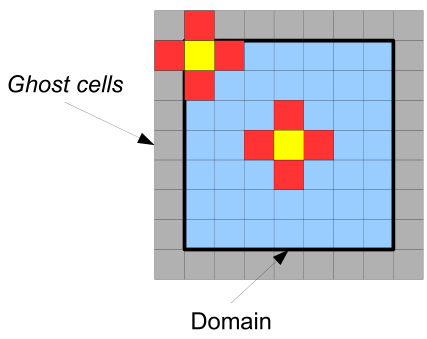
\includegraphics[scale=0.3]{./ghost-area.png}
  \caption{Rappresentazione della ghost area (celle
  grigie).}\label{fig:ghostarea}
\end{figure}

\subsection{Accesso in memoria al dominio}

È stato inizialmente ipotizzato l'accesso alla matrice considerandola come un
array, in accordo con la rappresentazione in memoria delle matrici fornita dal
linguaggio C.
Ciò avrebbe permesso di scorrere in modo sequenziale la matrice stessa,
risparmiando le chiamate alla funzione \texttt{IDX}.

Ad esempio, l'operazione di incremento di energia sarebbe stata implementata
come segue:
\begin{minted}{c}
for (int i = 0; i < n; i++) {
    grid[i] += delta;
}
\end{minted}

Tuttavia, l'introduzione della \textit{ghost area} ha reso preferibile (in
termini di gestione dell'accesso alla memoria) l'utilizzo della funzione
\texttt{IDX}, che contribuisce inoltre ad una buona comprensione e leggibilità
del codice sorgente.

\subsection{Versione OpenMP}

In figura \ref{fig:simulation1} è possibile osservare il risultato della
simulazione in termini di energia media delle celle e numero di celle che hanno
superato il valore soglia, misurate ad ogni passo di esecuzione.

\begin{figure}[!ht]
  \centering
  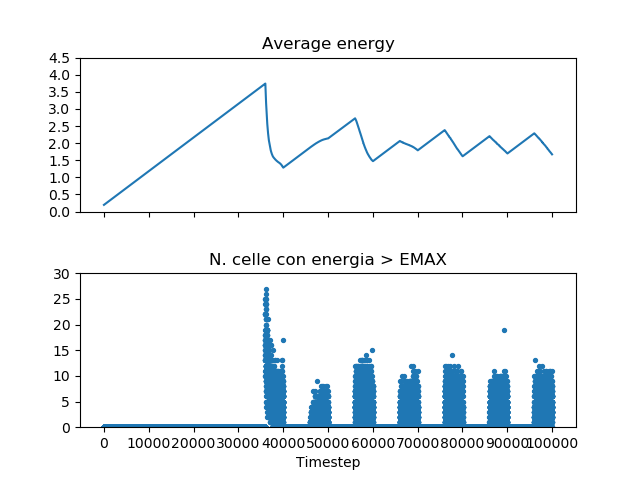
\includegraphics[scale=0.55]{./graphs/omp-earthquake.png}
  \caption{Energia media e numero di celle con energia maggiore di EMAX in un
  modello BK, n=256, 10\textsuperscript{5} timestep}\label{fig:simulation1}
\end{figure}

\subsubsection{Modifiche alla versione seriale}

\paragraph{setup}L'inizializzazione della ghost area a zero non è stata
parallelizzata poiché i test effettuati e mostrati nella tabella
\ref{tab:parallelghostarea} hanno evidenziato un degradamento, seppur minimo,
delle prestazioni.

\begin{table}[ht]
\centering
\begin{tabular}{rccc}
\cmidrule[\heavyrulewidth]{2-4}
 & Lato dominio & Numero passi & T\textsubscript{setup} (\textit{s})\\
 \cmidrule[\lightrulewidth]{2-4}
 seriale & \multirow{2}{*}{512} & \multirow{2}{*}{1000} & 0.00337177\\
 parallelizzato &&& 0.00454419\\
\cmidrule[\heavyrulewidth]{2-4}
\end{tabular}
\caption{\label{tab:parallelghostarea}Confronto dei tempi di esecuzione per la
funzione \texttt{setup} nella versione seriale e nella versione parallelizzata.}
\end{table}

Tale comportamento può essere dovuto ad un ulteriore carico di lavoro assegnato
allo scheduler per un'attività che mal si presta (soprattutto per l'accesso ai
lati sinistro e destro del dominio a causa dell'accesso in memoria) ad essere
parallelizzata.

\paragraph{altre operazioni}
Tutte le principali operazioni (incremento, conteggio, propagazione e calcolo
energia media) contengono dei cicli \texttt{for} che sono stati parallelizzati
utilizzando la direttiva OpenMP \texttt{omp parallel for}.  In tale modo
l'intero carico di lavoro del ciclo a cui è stato applicato il costrutto viene
suddiviso tra i thread che concorrono all'esecuzione del programma, realizzando
la vera e propria parallelizzazione.

Nelle operazioni di conteggio e di calcolo dell'energia media è stata inoltre
introdotta la clausola di riduzione con l'operatore somma, per poter
parallelizzare anche le operazioni di somma all'interno delle direttive OpenMP\@.

\subsubsection{Ulteriori ottimizzazioni}

\paragraph{collapse}

È stato valutato l'utilizzo della clausola \texttt{collapse(2)} sui cicli
\texttt{for} innestati per collassare le due iterazioni in una, allargando lo
spazio di iterazione come da specifiche\cite{openmp2018reference}.

Tale clausola ha tuttavia causato un degrado delle prestazioni (si veda la
tabella \ref{tab:collapse}) e pertanto non è stata implementata nella soluzione proposta.

\begin{table}[ht]
\begin{tabularx}{\linewidth}{rXXXXX}
\cmidrule[\heavyrulewidth]{2-6}
& Lato dom. & \# passi & $\overline{T}$\textsubscript{3-run}(\textit{s})
& cache-references (M/sec) & cache-misses (\%)*\\
\cmidrule[\lightrulewidth]{2-6}
senza \texttt{collapse(2)} & \multirow{2}{*}{256} & \multirow{2}{*}{100000} &
   13.33183 & 0.770 & 0.390\\
\cmidrule{4-6}
   con \texttt{collapse(2)} &&& 19.18336 & 0.560 & 0.402\\
\cmidrule[\heavyrulewidth]{2-6}
\end{tabularx}
\caption{\label{tab:collapse}Dati raccolti sull'esecuzione della simulazione con
e senza la direttiva \texttt{collapse(2)}.}
\end{table}

*: of all cache refs.

Dai dati presenti in tabella è possibile osservare che, al contrario di come ci
si aspetterebbe, nonostante la clausola \texttt{collapse} modifichi i
\textit{chunk} di memoria a cui si accede, ciò non comporta un degradamento
significativo delle prestazioni nell'accesso alla memoria cache.

Di conseguenza si ipotizza che l'incremento delle tempistiche di esecuzione
possa essere legato ad una cattiva gestione da parte dello scheduler
nell'organizzare il lavoro dei thread.

\paragraph{schedule}

È stata inoltre valutata l'adozione della clausola \texttt{schedule},
utilizzando il parametro \texttt{type} nelle sue varianti \texttt{static},
\texttt{dynamic} e \texttt{guided}.
%Si rimanda alle specifiche \cite{openmp2018reference} per ulteriori dettagli su
%tale operatore.

Le prove effettuate hanno mostrato un significativo aumento delle prestazioni
impostando uno scheduling statico con blocchi di dimensione 8.

La tabella \ref{tab:schedule} mostra la differenza di tempistiche medie (su 3
esecuzioni) tra la versione in cui la clausola \texttt{schedule} non è
specificata e quella in cui viene usata con parametri \texttt{static, 8}.

\begin{table}[ht]
\centering
\begin{tabularx}{400pt}{XXXX}
\toprule
Lato dom. & \# passi & $\overline{T}$\textsubscript{3-run}(\textit{s})&
$\overline{T}$\textsubscript{3-run}(\textit{s}) con \texttt{schedule(static,8)}\\
\midrule
 256 & \multirow{3}{*}{100000} & 12.9581 & 10.3148 \\
 512 && 50.4409 & 40.5048 \\
 1024 && 250.4084 & 177.2195 \\
\bottomrule
\end{tabularx}
\caption{\label{tab:schedule}Comparazione delle tempistiche di esecuzione
applicando uno scheduling statico.}
\end{table}

Tale clausola ha quindi permesso una importante riduzione delle tempistiche,
compresa tra il 20 e il 30\% in meno rispetto alla precedente versione già
parallelizzata.

Altri tipi di scheduling o diverse dimensioni dei \textit{chunk} hanno
pareggiato o addirittura peggiorato le precedenti tempistiche.

%Poiché le quattro operazioni fondamentali necessitano di essere eseguite in uno
%specifico ordine, non è stato possibile valutare altre ottimizzazioni o API
%di OpenMP per ottimizzare l'esecuzione.
%La principale è \texttt{parallel for}.

\subsection{Versione CUDA}

L'approccio all'implementazione della versione CUDA è stato più articolato,
poiché ha coinvolto l'inizializzazione e l'interazione con il dispositivo.
Di seguito si riporta il flusso di lavoro adottato nella programmazione della
versione CUDA della soluzione proposta:

\begin{enumerate}
    \item modifica delle operazioni dell'algoritmo: ogni funzione esprime il
        lavoro svolto dal singolo thread
    \item allocazione delle porzioni di memoria necessarie a contenere il
        dominio;
    \item partizionamento del dominio ed indicizzazione dei thread in accordo
        con il modello di suddivisione del carico di lavoro del dispositivo;
    \item inizializzazione del dominio e copia delle variabili nella memoria del
        dispositivo;
    \item esecuzione delle operazioni dell'algoritmo, se necesario
        sincronizzando i thread del dispositivo tra un'operazione e l'altra e
        scambiando i dati relativi all'esecuzione di una singola computazione
    \item deallocazione della memoria sia sull'\textit{host} che sul
        \textit{device}
\end{enumerate}

\subsubsection{Partizionamento del dominio}

Il dominio è stato partizionato, come da suggerimenti, in blocchi 2D organizzati
a loro volta in griglie 2D.

Per le operazioni effettuate nelle funzioni \texttt{count\_cells} e
\texttt{average\_energy} il dominio è stato invece partizionato in blocchi
monodimensionali, in accordo con la rappresentazione matriciale nel linguaggio
di programmazione C.

\subsubsection{Riduzione}

È stato inoltre adottato il pattern di riduzione con operazione somma mediante
l'API \texttt{atomicAdd}, di fatto interpretando le operazioni di conteggio e di
calcolo dell'energia media come somma degli elementi di un array.

%In un primo momento, per semplicità, si è proceduto con la realizzazione della
%soluzione senza l'utilizzo della memoria condivisa del Device.

%\newpage
\section{Valutazione prestazioni}
AMD Opteron (tm) Processor 6376 8 core 16 thread.


Le tempistiche indicate sono state tutte ottenute mediante le funzioni di
libreria messe a disposizione dal docente. Per ulteriori informazioni si
consulti il codice sorgente.

\subsection{Speedup}

Il calcolo dello speedup viene eseguito mediante la seguente formula:

\[ 
    S(p) = \frac{T_{serial}}{T_{parallel}(p)}
\]

in cui:
\begin{table}[ht]
\begin{tabular}{lll}
    p & : & \# processori/core\\
    T\textsubscript{serial}& : & tempo di esecuzione della porzione seriale
    (T\textsubscript{serial}=T\textsubscript{parallel}(1))\\
    T\textsubscript{parallel}(\textit{p}) & : & tempo di esecuzione della porzione con
    \textit{p} processori/core
\end{tabular}
\end{table}

Poiché l'implementazione della soluzione contiene porzioni di codice non
parallelizzabili (si veda la funzione \texttt{setup}), dovremmo considerare
T\textsubscript{parallel}(\textit{p}) nel seguente modo:

\[ 
T_{parallel}(p) = \alpha \cdot T_{serial} +  \frac{(1 - \alpha) \cdot
T_{serial}}{p}
\]

in cui $\alpha$ è il fattore relativo alla porzione di codice non
parallelizzabile, calcolato come segue:

\[ 
\alpha = \frac{T_{serial}}{T_{serial} + T_{parallel}}.
\]

Tuttavia, come mostrato nella seguente tabella, la porzione di codice seriale
(non parallelizzabile) impiega tempo trascurabile rispetto alla porzione di
codice parallelizzata, pertanto anche $\alpha$ assume valore trascurabile.

%\pgfmathparse{0.00140063/(0.00140063 + 14.2519)}\pgfkeys{/pgf/number format/sci}\pgfmathresult
\begin{table}[ht]
\begin{tabular}{ccccc}
\toprule
 Lato dominio & Numero passi & T\textsubscript{seriale} (\textit{s}) &
 T\textsubscript{parallelo} (\textit{s})& $\alpha$ \\
 \midrule
    256 & \multirow{2}{*}{100000} & 0.00140063 & 14.2519 & 0.00009827 \\
    1024 & & 0.02356447 & 150.2037 & 0.00015686 \\
\bottomrule
 %s_elapsed/(s_elapsed + p_elapsed)
 %0.00009827
\end{tabular}
\caption{caption}
\end{table}

Per le siffatte osservazioni, considereremo
T\textsubscript{parallel}(\textit{p}) in tal modo:

\[
T_{parallel}(p) = \frac{T_{serial}}{p}.
\]

\subsection{Strong scaling}

TODO

\subsection{Weak scaling}

TODO

\[
W(p) = \frac{T_{1}}{T_{p}}
\]

in cui:
\begin{table}[ht]
\begin{tabular}{lll}
    p &: & \# processori/core\\
    T\textsubscript{1}&: & tempo di esecuzione di una unità di lavoro con un
    processore/core\\
    T\textsubscript{p}&: & tempo di esecuzione di \textit{p} unità di lavoro con
    \textit{p} processori/core
\end{tabular}
\end{table}

%\newpage
\section{Conclusioni}

Tale relazione di progetto vuole portare all'attenzione tutte le fasi di
realizzazione del progetto stesso: l'analisi del modello, l'implementazione
delle versioni parallele e la valutazione delle prestazioni seguendo un
approccio quanto più metodico possibile.

Ogni sezione della relazione è inoltre accompagnata da considerazioni svolte
durante l'implementazione stessa, come, ad esempio, l'utilizzo di pattern,
clausole o l'adozione di una variante di una formula piuttosto che un'altra in
base a determinate condizioni. Tali scelte sono state inoltre motivate con dati
raccolti durante le varie verifiche in corso d'opera.

\subsection{Note di sviluppo}

Sono stati realizzati diversi script che facilitano ed automatizzano
l'esecuzione su server remoti e la valutazione delle prestazioni.

Possono risultare di interesse i meccanismi ideati per trasferire, compilare,
eseguire l'algoritmo e scaricare i risultati da/verso server remoti utilizzando
il comando \texttt{scp} e l'opzione \texttt{ProxyJump} di SSH.

In ultimo sono stati realizzati degli script per l'automatizzazione del calcolo
dei parametri prestazionali quali tempistiche, speedup e scalabilità.

Si consultino i sorgenti per maggiori informazioni.

\newpage
\appendix
%\section{Guida utente}


%\newpage
\bibliographystyle{plain}
\bibliography{./tex/bibliografia}
%\input{./tex/bibliografia.tex}

\end{document}
